\chapter{From Momentum Modes to Local Quantum Fields}

What is a quantum field, and how is it related to particles? The basic mathematical tool is the harmonic oscillator. A field contains many possible modes of oscillation, and quantizing the field amounts to putting together one quantum harmonic oscillator for each mode. The construction is easiest to see first in a finite periodic space, where the allowed modes form a discrete list.

\section{Periodic Space and Allowed Wave Numbers}

Take one spatial coordinate \(x\) and identify points separated by a distance \(L\). One can picture the space as a circle of circumference \(L\). This is a useful finite-volume trick. On a finite interval with endpoints, a traveling wave reflects from the ends. On a periodic interval it can continue in either direction without reflection. Translation symmetry, and therefore momentum conservation, is retained while the complications of infinite volume are temporarily removed.

A plane wave has the form
\begin{equation}
e^{ikx}.
\end{equation}
After one trip around the circle it must return to its original value. Since the wave equals \(1\) at \(x=0\), periodicity requires
\begin{equation}
e^{ikL}=1.
\end{equation}
Why does an integer multiple of \(2\pi\) solve this condition? Euler's formula gives
\begin{align}
e^{i2\pi n}
&=\cos(2\pi n)+i\sin(2\pi n)\\
&=1,
\qquad n\in\mathbb Z.
\end{align}
The cosine is \(1\) and the sine is \(0\) after any whole number of cycles. Consequently,
\begin{equation}
kL=2\pi n,
\qquad
k=\frac{2\pi n}{L},
\qquad n\in\mathbb Z.
\end{equation}
The quantity \(k\) is the wave number. The integer \(n\) labels an allowed wave number; it is not yet counting particles.

The same condition can be expressed in terms of wavelength. A wavelength is the distance through which the phase advances by one full cycle, so
\begin{equation}
k\lambda=2\pi,
\qquad
k=\frac{2\pi}{\lambda}.
\end{equation}
A long wavelength has a small wave number, and a short wavelength has a large wave number. The periodicity condition says that an integer number of wavelengths fits around the circle.

For a quantum-mechanical wave, the momentum is
\begin{equation}
p=\frac{h}{\lambda}
=\frac{2\pi\hbar}{\lambda}
=\hbar k.
\end{equation}
Thus \(k\) and \(p\) differ only by the factor \(\hbar\). Positive and negative \(k\) describe waves moving in opposite directions and particles with oppositely directed momentum. In units with \(\hbar=1\), it is common to call \(k\) the momentum without further distinction.

For every allowed \(k\), there may be some number of quanta in that mode. This introduces a second integer:
\begin{equation}
n(k)=\text{number of quanta with wave number }k.
\end{equation}
It is called the occupation number. The integer in \(k=2\pi n/L\) labels the mode; \(n(k)\) tells how many particles occupy that mode. Occupation numbers must be given for negative as well as positive \(k\).

\begin{classroomqa}
\lecturetimestamp{00:11:58}
\audiencequestion{Is \(k\) itself an integer?}
\lecturerresponse{No. The wave number is an integer multiple of \(2\pi/L\): \(k=2\pi n/L\). The integer \(n\) in that formula labels the allowed momentum, and it is distinct from the occupation number \(n(k)\), which counts quanta in the mode.}
\end{classroomqa}

\section{Occupation-Number States and Mode Operators}

A quantum state is a vector, or linear element. State vectors can be added and multiplied by numbers, and operators act on them to produce other state vectors. Observable real quantities are represented by Hermitian operators. These elementary facts matter here because both the many-particle state and the field will be built from linear combinations and operators.

Let
\begin{equation}
k_j=\frac{2\pi j}{L},
\qquad j\in\mathbb Z.
\end{equation}
A convenient label for a many-particle state is the entire string of occupation numbers,
\begin{equation}
\big|\{n(k_j)\}\big\rangle
=
\big|\ldots,n(k_{-2}),n(k_{-1}),n(k_0),n(k_1),n(k_2),\ldots\big\rangle.
\end{equation}
The entry \(n(k_1)\) is the number of particles in the first positive-momentum mode, \(n(k_2)\) is the number in the second, and so on. The string extends without end in both directions.

\begin{figure}[t]
\centering

\includegraphics[width=0.72\textwidth]{lecture_03_figure_02.png}
\caption{Occupation number \(n(k)\) for an allowed momentum mode.}
\lectureframe{00:15:04}
\end{figure}

Each momentum mode is a harmonic oscillator. It therefore has a raising operator and a lowering operator. The notation written initially as \(a^{+}(k)\) and \(a^{-}(k)\) will be written as \(a^\dagger(k)\) and \(a(k)\). Their actions are
\begin{align}
a^\dagger(k)\big|\ldots,n(k),\ldots\big\rangle
&=
\sqrt{n(k)+1}\,
\big|\ldots,n(k)+1,\ldots\big\rangle,
\\
a(k)\big|\ldots,n(k),\ldots\big\rangle
&=
\sqrt{n(k)}\,
\big|\ldots,n(k)-1,\ldots\big\rangle.
\end{align}
The operator \(a^\dagger(k)\) goes to the slot belonging to \(k\), raises that occupation by one, and multiplies the state by \(\sqrt{n(k)+1}\). The operator \(a(k)\) lowers the same slot and supplies \(\sqrt{n(k)}\). There is one such pair for every allowed momentum.

\begin{figure}[t]
\centering

\includegraphics[width=0.58\textwidth]{lecture_03_figure_03.png}
\caption{Creation and annihilation operators associated with momentum mode \(k\).}
\lectureframe{00:17:14}
\end{figure}

\section{Fourier Coefficients Become Operators}

The connection between these oscillator operators and a field begins with an ordinary classical Fourier series. A complex classical field on the periodic interval can be written
\begin{align}
\psi(x)&=\sum_k \alpha(k)e^{ikx},\\
\psi^*(x)&=\sum_k \alpha^*(k)e^{-ikx},
\end{align}
where every sum is over the allowed values \(k=2\pi n/L\). This is equivalent to expanding the field in sines and cosines.

The complex field has a real and an imaginary part. Its complex conjugate reverses the sign of the imaginary part, and \(e^{ikx}\) becomes \(e^{-ikx}\). Specifying all the coefficients \(\alpha(k)\) specifies the classical field. There is no need to specify \(\alpha^*(k)\) independently once \(\alpha(k)\) is known, but the real and imaginary parts of each coefficient are separate real quantities. They can be measured as the amplitudes of the corresponding Fourier components. In this sense a complex coefficient packages two classical observables.

Quantization replaces these classical Fourier coefficients by operators. An ordinary equality sign would identify objects of different kinds, so it is better to write a replacement rule:
\begin{equation}
\alpha(k)\rightsquigarrow a(k),
\qquad
\alpha^*(k)\rightsquigarrow a^\dagger(k).
\end{equation}
With a consistent choice of Fourier signs, the quantum fields are defined by
\begin{align}
\Psi(x)&=\sum_k a(k)e^{ikx},\\
\Psi^\dagger(x)&=\sum_k a^\dagger(k)e^{-ikx}.
\end{align}
\editorialnote{The spoken discussion changes and later questions the Fourier-sign convention. The conjugate pair used here is the convention visible in the clearer field expansion and in the position-state calculation: \(\Psi\) carries \(e^{ikx}\) and \(\Psi^\dagger\) carries \(e^{-ikx}\). Reversing every sign consistently would describe the same construction.}

For the moment, this is a definition: a quantum field is a Fourier sum whose coefficients are operators. A fuller justification would have to show how these operators reproduce the classical coefficients in an appropriate limit, which requires some dynamics. That question is postponed. What is already clear is that the field itself is an operator, and the relations among its Fourier coefficients are the creation-and-annihilation relations of harmonic oscillators.

\begin{classroomqa}
\lecturetimestamp{00:26:48}
\audiencequestion{Does introducing creation and annihilation operators mean that the dynamics necessarily creates and destroys particles?}
\lecturerresponse{No. The operators are mathematical operations that change occupation numbers. Whether the laws of nature actually change particle number is a question about the dynamics. If the dynamics permits such changes, these operators provide the natural language for describing them.}
\end{classroomqa}

\section{Scattering and Variable Particle Number}

First consider a process that does not change the number of particles. Suppose the only particle initially present has momentum \(k_7\). In occupation-number notation its state has a \(1\) in the seventh slot and zeros everywhere else:
\begin{equation}
|k_7\rangle
=
|\ldots,0,\underset{k_7}{1},0,\ldots\rangle.
\end{equation}
A scattering process changes its momentum from \(k_7\) to \(k_9\). The operator that makes exactly this change is
\begin{equation}
a^\dagger(k_9)a(k_7).
\end{equation}
The rightmost operator acts first: it removes the particle in the \(k_7\) slot. The left operator then creates a particle in the \(k_9\) slot.

\begin{classroomqa}
\lecturetimestamp{00:31:37}
\audiencequestion{Where do the square-root factors enter in this \(k_7\to k_9\) process?}
\lecturerresponse{The annihilation factor is \(\sqrt{n(k_7)}=\sqrt{1}=1\). After that removal the system is in the all-zero state. Since the \(k_9\) mode is empty, the creation factor is \(\sqrt{n(k_9)+1}=\sqrt{1}=1\). Thus neither factor changes the numerical coefficient in this one-particle example.}
\end{classroomqa}

Let us carry out both steps. Annihilation gives
\begin{align}
a(k_7)|k_7\rangle
&=
\sqrt{1}\,|\ldots,0,0,0,\ldots\rangle\\
&=|0\rangle.
\end{align}
The all-zero state is the vacuum. It is the state with no particles, and in this simple collection of oscillators it is also the ground state. Creation in the empty \(k_9\) mode then gives
\begin{equation}
a^\dagger(k_9)|0\rangle
=\sqrt{0+1}\,|k_9\rangle
=|k_9\rangle.
\end{equation}
Consequently,
\begin{equation}
a^\dagger(k_9)a(k_7)|k_7\rangle=|k_9\rangle.
\end{equation}
Slot by slot, the sole \(1\) has simply moved from the seventh momentum mode to the ninth. Because no occupation ever exceeded one, both square-root factors were equal to one. They will become important as soon as an already occupied mode is involved.

This one-to-one process could also be described in ordinary single-particle quantum mechanics: one particle changes its momentum. The occupation-number language becomes indispensable when particle number can change. For example,
\begin{equation}
a^\dagger(k_9)a^\dagger(k_{16})a(k_7)|k_7\rangle
=|k_9,k_{16}\rangle
\end{equation}
describes the mathematical change from one incoming particle in mode \(k_7\) to two outgoing particles, one in \(k_9\) and one in \(k_{16}\). A target may absorb the incoming particle, emit the two outgoing particles, and take up whatever recoil is required. Such a process cannot be represented in a Hilbert space restricted to one particle, but it fits naturally in a state space whose occupation numbers can vary. The operator expression is not by itself a law of nature; it is the language in which a number-changing law can be written.

\section{A Field Operator at a Point}

What does the position-space operator \(\Psi^\dagger(x)\) create? Quantum states form a linear space: momentum states may be added with complex coefficients to form a new state. Begin with the vacuum. Since every mode is empty,
\begin{equation}
\Psi(x)|0\rangle=0.
\end{equation}
The zero on the right is the zero vector: an annihilation operator cannot find any particle to remove.

The conjugate field acts differently:
\begin{align}
\Psi^\dagger(x)|0\rangle
&=\sum_k e^{-ikx}a^\dagger(k)|0\rangle\\
&=\sum_k e^{-ikx}|k\rangle,
\end{align}
where
\begin{equation}
|k\rangle=a^\dagger(k)|0\rangle
\end{equation}
is the one-particle state of momentum \(\hbar k\).

\begin{figure}[t]
\centering

\includegraphics[width=0.70\textwidth]{lecture_03_figure_05.png}
\caption{The formal position-space state \(\Psi^\dagger(x)|0\rangle\) expanded in one-particle momentum states.}
\lectureframe{00:43:16}
\end{figure}

Formally, and up to normalization, the sum is the generalized position state of one-particle quantum mechanics.\footnote{With infinitely many momentum modes, an exactly localized position state is non-normalizable. Imposing a finite momentum cutoff and normalizing the truncated sum instead gives a sharply localized wave packet centered at \(x\).} Momentum eigenstates, combined with coefficients \(e^{-ikx}\), produce localization at \(x\). In this formal sense,
\begin{equation}
\Psi^\dagger(x)\ \text{creates a particle at position }x,
\end{equation}
while
\begin{equation}
\Psi(x)\ \text{annihilates a particle at position }x.
\end{equation}
The mode operator \(a^\dagger(k)\) creates a particle with definite momentum. The field operator \(\Psi^\dagger(x)\) creates the coherent superposition of allowed momentum states that is formally localized at \(x\).

In the formal, unnormalized sum, every coefficient \(e^{-ikx}\) has magnitude one. With a finite cutoff, the normalized truncated state has equal-magnitude coefficients for the retained momenta, while their phases produce a wave packet sharply localized near \(x\). This is the elementary connection between a quantum field and particles.

Ignoring special-relativistic complications for now, \(\Psi^\dagger(x)\) creates a particle at \(x\) in this model. Relativistic fields require refinements, but the operator-valued Fourier expansion and the distinction between momentum-mode and position-space operators remain basic.

\begin{classroomqa}
\lecturetimestamp{00:44:59}
\audiencequestion{Is \(x\) a spot on the periodic circle, and what happens as the circle becomes large?}
\lecturerresponse{Yes. In the finite model, \(x\) is a point on the circle. Neighboring allowed wave numbers are separated by \(2\pi/L\). As \(L\) grows, that spacing becomes smaller, so for every desired momentum there is an allowed value arbitrarily close to it. In the infinite-volume limit, sums over \(k\) are replaced by integrals over \(k\). It is useful to understand the discrete sums first.}
\end{classroomqa}

\section{Local Particle Reactions}

Once \(\Psi(x)\) and \(\Psi^\dagger(x)\) have been interpreted as annihilating and creating particles at a point, locality can be expressed directly. Imagine that a particle is absorbed by a target sharply localized at \(x\), while one outgoing particle suddenly appears near Alpha Centauri and another near Betelgeuse. Such a reaction is nonlocal: its separated events cannot be connected by ordinary propagation.

One could first weaken the requirement and allow the outgoing particles to be emitted somewhere within a small region around the target. The precise local idealization is stronger: if the incoming particle is absorbed at \(x\), the outgoing particles are created at that same point. Using fields evaluated at separated points would instead describe a nonlocal operator product. A local one-to-two operation is therefore
\begin{equation}
\Psi^\dagger(x)\Psi^\dagger(x)\Psi(x).
\end{equation}
The rightmost field removes the incoming particle at \(x\); the two fields to its left create two outgoing particles there.\footnote{The local one-to-two schematic follows the reaction described at 00:47:38--00:49:13.}

\begin{figure}[t]
\centering
\begin{tikzpicture}[scale=1.0]
\draw[->] (-2.2,0) -- (0,0);
\fill (0,0) circle (2.2pt);
\draw[->] (0,0) -- (2.0,1.1);
\draw[->] (0,0) -- (2.0,-1.1);
\node at (-1.25,0.3) {$k_{\mathrm{initial}}$};
\node[right] at (0.05,0.05) {$x$};
\node at (1.48,1.34) {$\ell$};
\node at (1.48,-1.34) {$m$};
\end{tikzpicture}
\caption{One incoming particle is absorbed at \(x\), and two outgoing particles are created at the same point.}
\end{figure}

Let the incoming state contain one particle of definite wave number \(k_{\mathrm{initial}}\). To determine the outgoing momenta, substitute the momentum-space expansions of the local fields. It is important to separate a fixed momentum label from a dummy summation index. Write
\begin{align}
\Psi(x)&=\sum_q a(q)e^{iqx},\\
\Psi^\dagger(x)&=\sum_\ell a^\dagger(\ell)e^{-i\ell x}.
\end{align}
The index \(q\) is summed, whereas \(k_{\mathrm{initial}}\) labels the particular occupied incoming mode. The two copies of \(\Psi^\dagger(x)\) also require independent dummy indices, say \(\ell\) and \(m\). Reusing one index would incorrectly tie two independent sums together. Here \(\ell\) and \(m\) are wave numbers; \(m\) does not denote mass.

A concrete picture is a photon striking an atom localized at \(x\), followed by two photons leaving that point. The simple field used here is better suited to nonrelativistic particles than to a fully relativistic photon field, so the photon language is only illustrating the operator bookkeeping.

The annihilation field acts first:
\begin{align}
\Psi(x)|k_{\mathrm{initial}}\rangle
&=\sum_q e^{iqx}a(q)a^\dagger(k_{\mathrm{initial}})|0\rangle.
\end{align}
Every term vanishes except the one with \(q=k_{\mathrm{initial}}\). An annihilation operator has to find a particle in its own mode. Hence
\begin{equation}
\Psi(x)|k_{\mathrm{initial}}\rangle
=e^{ik_{\mathrm{initial}}x}|0\rangle.
\end{equation}
The two creation fields then give
\begin{align}
&\Psi^\dagger(x)\Psi^\dagger(x)\Psi(x)
|k_{\mathrm{initial}}\rangle
\\
&\quad=
e^{ik_{\mathrm{initial}}x}
\sum_{\ell,m}
e^{-i\ell x}e^{-imx}
a^\dagger(\ell)a^\dagger(m)|0\rangle
\\
&\quad=
\sum_{\ell,m}
e^{i(k_{\mathrm{initial}}-\ell-m)x}
a^\dagger(\ell)a^\dagger(m)|0\rangle.
\end{align}
For unequal \(\ell\) and \(m\), the operator state may be denoted \(|\ell,m\rangle\): one particle occupies each of the two modes. The final result is a sum over all such two-particle momentum configurations, with a phase determined by the incoming and outgoing momenta.

\begin{classroomqa}
\lecturetimestamp{01:00:36}
\audiencequestion{Do the two creation operators commute?}
\lecturerresponse{Yes. All creation operators commute with one another, and all annihilation operators commute with one another. A creation and an annihilation operator commute when they refer to different modes; for the same mode their commutator is nonzero.}
\end{classroomqa}

\begin{classroomqa}
\lecturetimestamp{01:01:34}
\audiencequestion{Should the two outgoing momenta satisfy momentum conservation?}
\lecturerresponse{The displayed particles need not conserve momentum by themselves because the atom or target can recoil. The difference \(k_{\mathrm{initial}}-\ell-m\) is the momentum transferred to the target. Total momentum, including the target, is the conserved quantity.}
\end{classroomqa}

Since the coefficient \(e^{i(k_{\mathrm{initial}}-\ell-m)x}\) is a pure phase, its magnitude is one. At first sight this suggests equal probability weights for all pairs \((\ell,m)\). There is, however, an important qualification when the two labels coincide.

If \(\ell=m\), the first creation operator puts one particle in mode \(m\), and the second acts on a mode already occupied once:
\begin{align}
a^\dagger(m)a^\dagger(m)|0\rangle
&=a^\dagger(m)|1_m\rangle\\
&=\sqrt{2}\,|2_m\rangle.
\end{align}
Thus double creation in one mode has an extra amplitude \(\sqrt{2}\). Squaring an amplitude produces a factor of \(2\) in probability.

\begin{classroomqa}
\lecturetimestamp{01:04:54}
\audiencequestion{Must \(\ell\) and \(m\) differ by one because the creation coefficient contains \(n+1\)?}
\lecturerresponse{No. The symbols \(\ell\) and \(m\) label momentum modes. The \(n\) in \(\sqrt{n+1}\) is the occupation number of the particular mode on which the creation operator acts. Momentum labels and particle counts are distinct integers.}
\end{classroomqa}

\begin{figure}[t]
\centering

\includegraphics[width=0.92\textwidth]{lecture_03_figure_06.png}
\caption{Momentum-space expansion of the local one-to-two particle amplitude.}
\lectureframe{01:05:44}
\end{figure}

The particles in this construction are identical. The \(\sqrt{2}\) is therefore a bosonic occupation factor, not a label distinguishing a first particle from a second. Squaring it seems, provisionally, to make the same-momentum outcome twice as probable as a single unequal-momentum term. That comparison will need another look once the terms in the double sum are counted carefully.

\begin{classroomqa}
\lecturetimestamp{01:06:43}
\audiencequestion{In a complicated reaction, how is the order of creation and annihilation operators chosen?}
\lecturerresponse{An expression with all creation operators to the left and annihilation operators to the right is called normal ordered. In that form the rightmost operators first remove incoming particles and the remaining operators create outgoing particles.}
\end{classroomqa}

Reordering a mixed creation--annihilation pair is not generally a simple permutation: it must use the commutator, and for the same mode this produces an additional term.\footnote{This commutator qualification is an editorial correction to the informal normal-ordering discussion at 01:06:43.}

\begin{classroomqa}
\lecturetimestamp{01:07:30}
\audiencequestion{If the momentum amplitudes all have the same magnitude, what does a statement such as ``twice as probable'' mean?}
\lecturerresponse{Keep the finite cavity in mind. Its allowed momenta are discrete, so probabilities can be compared mode by mode. The comparison is not between probabilities of isolated points in a continuum.}
\end{classroomqa}

For \(\ell\ne m\), the unrestricted double sum contains both ordered terms
\begin{equation}
a^\dagger(\ell)a^\dagger(m)|0\rangle
\quad\text{and}\quad
a^\dagger(m)a^\dagger(\ell)|0\rangle.
\end{equation}

\begin{classroomqa}
\lecturetimestamp{01:08:24}
\audiencequestion{When \(\ell\ne m\), does the same final state occur twice in the double sum, once as \((\ell,m)\) and once as \((m,\ell)\)?}
\lecturerresponse{Yes. If \(\ell\ne m\), the terms \((\ell,m)\) and \((m,\ell)\) both occur, and because the creation operators commute they describe the same physical state.}
\end{classroomqa}

The two ordered terms are equal, so state normalization and this double counting must be handled before a quantitative channel comparison is made. The reliable algebraic conclusion is narrower and sufficient for what follows: creating in a mode already occupied by \(n\) identical bosons produces the factor \(\sqrt{n+1}\).

\section{Spontaneous and Stimulated Emission}

A cleaner example isolates the square-root factor. Suppose an object localized at \(x\) emits one photon. If the photon field begins in the vacuum, the outgoing state is
\begin{align}
\Psi^\dagger(x)|0\rangle
&=\sum_k e^{-ikx}a^\dagger(k)|0\rangle\\
&=\sum_k e^{-ikx}|k\rangle.
\end{align}
Within this simplified model all momenta have equal amplitude magnitude. With no photons already present, the emission is spontaneous.

Now suppose there is already one photon in mode \(\ell\). Acting with the same local creation field gives two kinds of terms:
\begin{equation}
\Psi^\dagger(x)|\ell\rangle
=
\sum_{k\ne\ell}e^{-ikx}|k,\ell\rangle
+e^{-i\ell x}\sqrt{2}\,|2_\ell\rangle.
\end{equation}
For \(k\ne\ell\), the operator creates into an empty mode, so the coefficient is \(\sqrt{0+1}=1\). For \(k=\ell\), it creates into the occupied mode, so the coefficient is \(\sqrt{1+1}=\sqrt{2}\). The original photon is a bystander; the new photon is preferentially emitted into its occupied mode.

\begin{classroomqa}
\lecturetimestamp{01:16:14}
\audiencequestion{Must the pre-existing photon be at the same location in order to stimulate the emission?}
\lecturerresponse{The simplified calculation refers to occupation of the same momentum mode, not to two particles at one sharply defined position. A particle cannot have both exact position and exact momentum. Real photons are described by wave packets, while the cavity idealization provides definite discrete modes. In that setting the enhancement is into the already occupied cavity mode.}
\end{classroomqa}

If mode \(\ell\) initially contains \(n_\ell\) photons, then
\begin{equation}
a^\dagger(\ell)
|\ldots,n_\ell,\ldots\rangle
=
\sqrt{n_\ell+1}
\,|\ldots,n_\ell+1,\ldots\rangle.
\end{equation}
The probability is therefore enhanced by the factor \(n_\ell+1\). With one photon already present the factor is \(2\). With one hundred photons in the mode, the amplitude factor is \(\sqrt{101}\), and the probability for emission into that mode is \(101\) times the empty-mode value. The more quanta already present in a bosonic mode, the more likely the next quantum is to be emitted into that mode. This is stimulated emission.

The same occupation effect appears in scattering reactions. If a collision can produce a particle in several modes, pre-existing occupation enhances production into the occupied modes. It is a general property of this oscillator algebra, not a special peculiarity of atomic decay.

\begin{classroomqa}
\lecturetimestamp{01:18:15}
\audiencequestion{In the earlier two-particle process, do two newly created particles still carry greater weight when their momenta differ?}
\lecturerresponse{Yes. In the ordered double sum, an unequal-momentum pair occurs in two orders. The same-mode factor \(\sqrt{2}\) reduces that combinatorial difference, but by itself does not erase it.}
\end{classroomqa}

As before, a physical channel comparison still requires consistent state normalization and counting.

\begin{classroomqa}
\lecturetimestamp{01:18:30}
\audiencequestion{Does that mean bosons are attracted toward already occupied momentum states?}
\lecturerresponse{No. There is no literal force or attraction. The enhancement is a statistical consequence of particle identity and the square-root factors in the bosonic creation operators.}
\end{classroomqa}

It is useful to keep the two names separate. If no photons are present, the coefficient begins with \(n=0\), giving the unit factor associated with spontaneous emission. If photons are already present, the factor \(n+1\) makes emission into their mode more likely; that is stimulated emission.

There is a classical analog. A pre-existing electromagnetic wave passing an atom drives its electrons. The driven electrons radiate more strongly than they would without the wave, and the added radiation follows the direction and wave number of the driving wave. The quantum statement replaces the pre-existing wave by occupied photon modes: existing quanta stimulate the production of more quanta in the same mode.

Particles governed by this harmonic-oscillator algebra are bosons. They have a statistical tendency to accumulate in occupied states, though they do not attract one another into those states. Particles come in two statistical kinds, bosons and fermions. The present construction is bosonic; the opposite fermionic behavior is taken up later.

\section{Bosonic Algebra and Particle Density}

For every momentum mode there are creation and annihilation operators. Their algebra is
\begin{align}
[a^\dagger(k),a^\dagger(\ell)]&=0,\\
[a(k),a(\ell)]&=0,\\
[a(k),a^\dagger(\ell)]&=\delta_{k\ell}.
\end{align}
Here
\begin{equation}
[A,B]=AB-BA,
\end{equation}
and the Kronecker delta is
\begin{equation}
\delta_{k\ell}=
\begin{cases}
1,&k=\ell,\\
0,&k\ne\ell.
\end{cases}
\end{equation}
Creation operators commute for equal or unequal momenta, as do annihilation operators. A mixed pair commutes for different momenta; for the same momentum it has the familiar single-oscillator commutator.

Together with the Fourier definition of \(\Psi(x)\), these relations define the simplest bosonic quantum field. The field's work is to create and annihilate particles, mode by mode or at specified positions.

Consider now the operator
\begin{equation}
\int_0^L dx\,\Psi^\dagger(x)\Psi(x).
\end{equation}
Instead of naming it in advance, work it out. Substitution of the Fourier expansions gives
\begin{align}
\int_0^L dx\,\Psi^\dagger(x)\Psi(x)
&=
\sum_{k,\ell}a^\dagger(k)a(\ell)
\int_0^L dx\,e^{-ikx}e^{i\ell x}
\\
&=
\sum_{k,\ell}a^\dagger(k)a(\ell)
\int_0^L dx\,e^{i(\ell-k)x}.
\end{align}
If \(k=\ell\), the exponential is \(1\) and the integral is \(L\). If \(k\ne\ell\), an integer number of sine and cosine cycles is integrated around the circle; positive and negative parts cancel. Thus
\begin{equation}
\int_0^L dx\,e^{i(\ell-k)x}=L\delta_{k\ell}.
\end{equation}
The double sum collapses to
\begin{equation}
\int_0^L dx\,\Psi^\dagger(x)\Psi(x)
=L\sum_k a^\dagger(k)a(k).
\end{equation}
For each mode,
\begin{equation}
a^\dagger(k)a(k)=N_k
\end{equation}
is the occupation-number operator. Summing it counts all particles:
\begin{equation}
N=\sum_k N_k=\sum_k a^\dagger(k)a(k).
\end{equation}
With the present Fourier normalization,
\begin{equation}
N=\frac{1}{L}\int_0^L dx\,
\Psi^\dagger(x)\Psi(x).
\end{equation}
Other conventions put factors such as \(1/\sqrt{L}\) into the Fourier expansion and remove the explicit \(1/L\) here. In the convention being used, the local number-density operator is
\begin{equation}
\rho(x)=\frac{1}{L}\Psi^\dagger(x)\Psi(x),
\qquad
\int_0^L dx\,\rho(x)=N.
\end{equation}
Thus \(\Psi^\dagger(x)\Psi(x)\) is proportional to particle density. Calling it the number of particles at one mathematical point is misleading; density is the appropriate local notion.

The total number may or may not be conserved. If the dynamics creates or absorbs particles, \(N\) can change with time. If particle number is conserved by the dynamics, then \(N\) is a conserved observable.

Knowing the commutators of the mode operators also makes it possible to work out the commutators of \(\Psi(x)\) and \(\Psi^\dagger(x)\). That calculation is left as a useful exercise in applying the Fourier sums.

This construction describes one species of identical bosons. Identical means that all the particles are of the same kind, though they may have different positions and momenta. One would not put electrons and photons into the same field \(\Psi\). A photon field requires relativistic refinements to this elementary model. An electron field requires a different, fermionic algebra.

\begin{classroomqa}
\lecturetimestamp{01:35:43}
\audiencequestion{Is this construction only one-dimensional?}
\lecturerresponse{The example so far has one spatial coordinate, but nothing essential depends on that. Higher dimensions are obtained by introducing additional coordinates and momentum components.}
\end{classroomqa}

\editorialnote{A brief exchange here appears to begin with fluorescence and stimulated emission, then turns to transparency and interference. The damaged wording does not support a reliable reconstruction of the question or its answer.}

Examples include photons, the Higgs boson, and gravitons.\footnote{Other particle names in the brief example list are indistinct and are not retained.}

\section{Large Occupation and the Classical Field Limit}

A complex field operator is not itself a single Hermitian observable. Its two Hermitian components are
\begin{equation}
\Psi_1(x)=\frac{\Psi(x)+\Psi^\dagger(x)}{2},
\qquad
\Psi_2(x)=\frac{\Psi(x)-\Psi^\dagger(x)}{2i}.
\end{equation}
They are the quantum analogs of the real and imaginary parts of a classical field. They do not commute, so both cannot be measured simultaneously with arbitrary precision. This is the field version of the uncertainty between the conjugate variables of a harmonic oscillator.

When, then, can the field behave like a classical wave? Consider one highly excited momentum mode \(k\). Its number operator is
\begin{equation}
a^\dagger(k)a(k)=N_k.
\end{equation}
Suppose the state has a large mean occupation, \(\langle N_k\rangle=n_k\gg 1\). The scale available to a macroscopic oscillator amplitude is then of order \(\sqrt{n_k}\). Meanwhile, the right-hand side of
\begin{equation}
[a(k),a^\dagger(k)]=1
\end{equation}
remains fixed. The commutator never vanishes, but at large occupation its effects can be small compared with the squared scale of the excitation. Large occupation supplies the scale needed for a classical limit, but it is not sufficient by itself. The state must also be appropriately phase coherent, so that the uncertainties of the two quadratures are small compared with the macroscopic field amplitude.\footnote{This qualifies the large-occupation heuristic. A number eigenstate has \(\langle a(k)\rangle=0\), no definite phase, and quadrature fluctuations of order \(\sqrt{n_k}\); it is not by itself a classical wave.}

For an electromagnetic field, large occupation means many photons. In an appropriately phase-coherent state with many photons in the relevant modes, the measurable field components behave approximately like an ordinary classical electromagnetic wave. With only a few photons, the discreteness of the quanta is visible and the classical wave description fails. A quantum field remains an operator in both regimes; what changes is the relative importance of its quantum fluctuations.

\begin{classroomqa}
\lecturetimestamp{01:42:09}
\audiencequestion{Is the large occupation number the initial occupation or the final occupation?}
\lecturerresponse{If the process changes the number of photons only slightly, it does not matter for this argument. The initial and final occupations are both large, and their difference is small compared with either one.}
\end{classroomqa}

The opposite extreme is the ground state, in which every occupation number is zero. That state is highly quantum mechanical, and its notation must be distinguished carefully from the null vector.

\begin{classroomqa}
\lecturetimestamp{01:42:36}
\audiencequestion{If an annihilation operator acts on the vacuum, does it produce the vacuum again, or no state at all?}
\lecturerresponse{It produces the zero vector, \(a(k)|0\rangle=\mathbf{0}\). The vacuum \(|0\rangle\) is a genuine normalized state with no particles, satisfying \(\langle0|0\rangle=1\). It is not the zero vector. The zero vector has zero norm and represents no physical state.}
\end{classroomqa}

\begin{classroomqa}
\lecturetimestamp{01:44:11}
\audiencequestion{Is the field itself another kind of state?}
\lecturerresponse{No. In quantum field theory the field is an operator. States are vectors, and the field operators act on those vectors.}
\end{classroomqa}

\section{Periodic Space in Practice}

The periodic construction is a calculational device rather than a claim that the universe is literally a circle of some chosen circumference. Closely related discrete-mode systems do occur in practice.

\begin{classroomqa}
\lecturetimestamp{01:45:03}
\audiencequestion{How is the finite periodic model used in practice?}
\lecturerresponse{Radiation in a cavity with reflecting walls provides a familiar discrete set of modes. A particle moving around a closed wire gives a directly periodic example. Taking \(L\) to be the size of the universe is neither necessary nor especially useful.}
\end{classroomqa}

Fixing \(L\) gives a nonzero separation between adjacent momenta, but it does not leave only finitely many of them.

\begin{classroomqa}
\lecturetimestamp{01:45:39}
\audiencequestion{Does fixing the length \(L\) limit the total number of possible momentum states?}
\lecturerresponse{No. The allowed values are \(k_j=2\pi j/L\), and \(j\) can be any integer, so there are still infinitely many modes. Finite \(L\) gives only finitely many modes below a chosen maximum momentum. Without such a cutoff, the momentum label remains unbounded.}
\end{classroomqa}

The oscillator interpretation can also be read in reverse. In elementary oscillator mechanics one begins with conjugate variables and constructs \(a\) and \(a^\dagger\). Here the mode operators were introduced first, so it is natural to ask where their conjugate variables appear.

\begin{classroomqa}
\lecturetimestamp{01:46:43}
\audiencequestion{For a fixed mode, what corresponds to the oscillator variables \(X\) and \(P\) when the construction begins with \(a(k)\) and \(a^\dagger(k)\)?}
\lecturerresponse{For each fixed momentum mode there is one oscillator. Its two Hermitian quadratures are built from \(a(k)\) and \(a^\dagger(k)\), just as the real and imaginary field components are built from \(\Psi\) and \(\Psi^\dagger\). Up to normalization and a possible interchange of names, these are the analogs of \(X\) and \(P\).}
\end{classroomqa}

For the fixed mode, suppressing convention-dependent numerical factors, the quadratures are\footnote{The exchange at 01:46:43 moves loosely between one momentum mode and the full field. The displayed relation makes the fixed-mode statement explicit: \(\Psi(x)\) and \(\Psi^\dagger(x)\) are Fourier sums over all modes.}
\begin{equation}
X_k\propto a(k)+a^\dagger(k),
\qquad
P_k\propto \frac{a(k)-a^\dagger(k)}{i}.
\end{equation}
The position-space components \(\Psi_1(x)\) and \(\Psi_2(x)\) introduced above are Fourier superpositions of these mode quadratures, not the quadratures of one fixed mode. Their uncertainty relation is the same obstruction encountered when trying to regard a weakly excited quantum field as a completely classical object.

\section{Periodic Space in Higher Dimensions}

\begin{classroomqa}
\lecturetimestamp{01:48:21}
\audiencequestion{How is periodic space represented in more than one dimension?}
\lecturerresponse{In two dimensions the analog of the circle is a torus. It can be represented by a rectangle whose left and right edges are identified and whose bottom and top edges are identified. There are two periodic directions, so both momentum components are quantized.}
\end{classroomqa}

A torus is often pictured as the surface of a doughnut, but a rectangle is more useful for calculation. Cut the surface once and open it into a cylinder. Cut the cylinder once more and lay it flat. The resulting rectangle still carries two identifications: the left edge is the same as the right edge, and the bottom edge is the same as the top edge.\footnote{The rectangle, its two edge identifications, the reappearing particle, and the statement that both momentum components are quantized follow 01:48:46--01:50:58. The displayed formulas for \(k_x\) and \(k_y\) are the componentwise reconstruction of the earlier condition \(kL=2\pi n\).}

A particle that crosses the right edge reappears at the corresponding point on the left. If it crosses the top, it reappears at the corresponding point on the bottom. A periodic field obeys
\begin{align}
\Psi(x+L_x,y)&=\Psi(x,y),\\
\Psi(x,y+L_y)&=\Psi(x,y).
\end{align}
For a plane wave \(e^{i(k_x x+k_y y)}\), these identifications require
\begin{equation}
k_x=\frac{2\pi n_x}{L_x},
\qquad
k_y=\frac{2\pi n_y}{L_y},
\qquad
n_x,n_y\in\mathbb Z.
\end{equation}
Both components of momentum are discrete.

\begin{figure}[t]
\centering
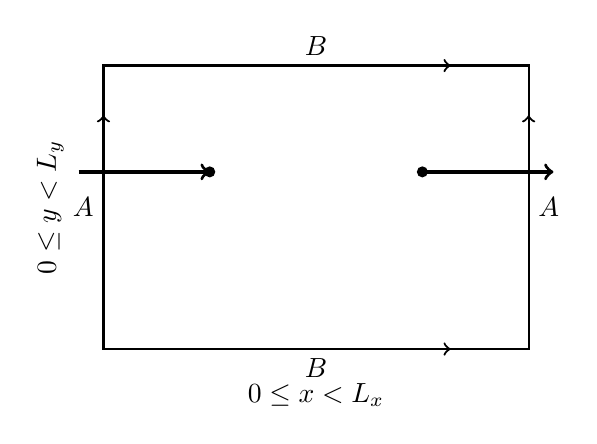
\begin{tikzpicture}[x=0.9cm,y=0.9cm]
\draw[thick] (0,0) rectangle (6,4);
\draw[->,thick] (0,0.7) -- (0,3.3);
\draw[->,thick] (6,0.7) -- (6,3.3);
\draw[->,thick] (1.1,0) -- (4.9,0);
\draw[->,thick] (1.1,4) -- (4.9,4);
\node[left] at (0,2) {$A$};
\node[right] at (6,2) {$A$};
\node[below] at (3,0) {$B$};
\node[above] at (3,4) {$B$};
\draw[->,very thick] (4.5,2.5) -- (6.35,2.5);
\draw[->,very thick] (-0.35,2.5) -- (1.5,2.5);
\fill (4.5,2.5) circle (2pt);
\fill (1.5,2.5) circle (2pt);
\node at (3,-0.65) {$0\leq x<L_x$};
\node[rotate=90] at (-0.75,2) {$0\leq y<L_y$};
\end{tikzpicture}
\caption{A two-dimensional periodic space: edges carrying the same label are identified, so a particle crossing one edge reappears at the corresponding point on the opposite edge.}
\end{figure}

\begin{classroomqa}
\lecturetimestamp{01:50:58}
\audiencequestion{Does the periodic construction represent space, or the objects in space?}
\lecturerresponse{It represents space. The objects and fields live in that space and obey its identifications. Periodicity is imposed to control the infinite-volume problem; it is removed by taking the volume large and replacing momentum sums by integrals.}
\end{classroomqa}

The three-dimensional analog is a cube with three pairs of opposite faces identified. The left and right faces are the same, the top and bottom faces are the same, and the front and back faces are the same. A particle crossing any face reappears through its identified partner.\footnote{The periodic cube and its three pairs of identified faces follow 01:51:27--01:52:17. The displayed equation for \(k_i\) is the componentwise reconstruction of the earlier condition \(kL=2\pi n\), applied to the three periodic directions.} The three momentum components obey
\begin{equation}
k_i=\frac{2\pi n_i}{L_i},
\qquad i=x,y,z,
\end{equation}
with one integer \(n_i\) for each direction. Tori can be defined in any number of dimensions by the same rule.

\begin{figure}[t]
\centering
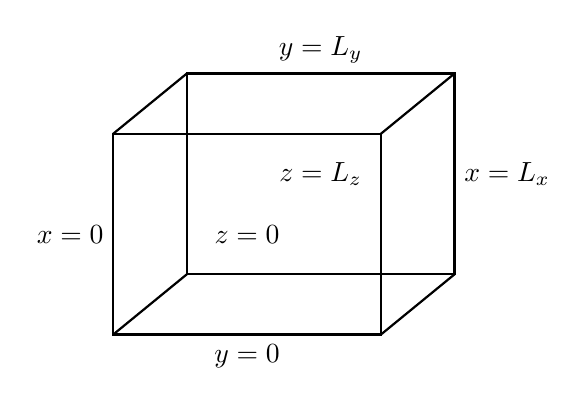
\begin{tikzpicture}[scale=0.85]
\draw[thick] (0,0) rectangle (4,3);
\draw[thick] (1.1,0.9) rectangle (5.1,3.9);
\draw[thick] (0,0) -- (1.1,0.9);
\draw[thick] (4,0) -- (5.1,0.9);
\draw[thick] (4,3) -- (5.1,3.9);
\draw[thick] (0,3) -- (1.1,3.9);
\node[left] at (0,1.5) {$x=0$};
\node[right] at (5.1,2.4) {$x=L_x$};
\node[below] at (2,0) {$y=0$};
\node[above] at (3.1,3.9) {$y=L_y$};
\node at (2,1.5) {$z=0$};
\node at (3.1,2.4) {$z=L_z$};
\end{tikzpicture}
\caption{A three-dimensional periodic space as a cube with each pair of opposite faces identified.}
\end{figure}

\begin{classroomqa}
\lecturetimestamp{01:52:20}
\audiencequestion{Does field theory choose a physical grid size for space?}
\lecturerresponse{That is a speculative question. For practical purposes here, space is continuous. The quanta are particles, not cells of a spatial grid. In the circle construction it is momentum that becomes discrete; position remains continuous and periodic.}
\end{classroomqa}

\editorialnote{A long damaged passage during the grid-size exchange mentions Planckian scales but does not preserve a recoverable claim about fundamental spatial discreteness. No such claim is inferred here.}

The discreteness of \(k\) came entirely from imposing a periodic wave function. It is not evidence that the coordinate \(x\) itself lies on a lattice. Questioning whether space may have a fundamental microscopic structure is legitimate, but it is a separate, speculative issue.

\section{Fermions and External Fields}

Bosonic modes allow any nonnegative occupation number. Fermions require the opposite behavior: the Pauli exclusion principle forbids two identical fermions from occupying the same state.

\begin{classroomqa}
\lecturetimestamp{01:55:13}
\audiencequestion{Does replacing commutators by anticommutators give the simplest fermion theory?}
\lecturerresponse{Yes, in essence. The commutator is \([A,B]=AB-BA\), whereas the anticommutator is \(\{A,B\}=AB+BA\). The corresponding fermionic creation-and-annihilation algebra implements Pauli exclusion: a second identical fermion cannot be put into an already occupied state. The detailed theory is deferred.}
\end{classroomqa}

The two products differ by a sign:
\begin{equation}
[A,B]=AB-BA,
\qquad
\{A,B\}=AB+BA.
\end{equation}
The commutator is antisymmetric under exchange, while the anticommutator is symmetric. If an anticommutator vanishes, then
\begin{equation}
\{A,B\}=0
\quad\Longrightarrow\quad
AB=-BA.
\end{equation}
For such a pair, exchanging the two fermionic operators changes the sign. This is more unusual than ordinary commuting, where \([A,B]=0\) gives \(AB=BA\). Replacing the bosonic commutators by the corresponding anticommuting algebra is the mathematical change that leads to fermions; its detailed development is postponed.

Anticommutation reverses the statistical behavior seen for bosons. There is no stimulated piling-up of identical fermions in one mode; occupancy of that mode blocks another identical fermion from entering it. Since a single fermionic state can contain at most one identical fermion, no classical field limit is obtained by putting an arbitrarily large number of them into that one state.

\begin{classroomqa}
\lecturetimestamp{01:58:03}
\audiencequestion{How can an alpha particle be a boson if it is made from fermions?}
\lecturerresponse{A bound composite containing an even number of fermionic constituents can have bosonic statistics. Putting several such composite bosons into the same overall state is not the same as putting their individual fermionic constituents into one identical single-particle state.}
\end{classroomqa}

Composite statistics concern the bound object as a whole. Fermionic constituents can therefore combine into an object that behaves as a boson without violating exclusion for the constituents.

\begin{classroomqa}
\lecturetimestamp{01:58:33}
\audiencequestion{How are external fields incorporated?}
\lecturerresponse{No external background field has been included in the construction so far. Such a field can be prescribed as a classical field, or represented quantum mechanically by a state containing a large number of quanta.}
\end{classroomqa}

For the two descriptions to agree, the large-occupation state must be appropriately prepared and phase coherent; particle number alone is not sufficient.\footnote{The exchange supplies the many-quanta scale. Phase coherence is stated here as the additional condition that prevents large occupation alone from being mistaken for a classical field.} In that semiclassical regime their effects agree up to small quantum deviations. This is a basic consistency condition. The electromagnetic field must describe discrete photons when individual quanta matter, yet an appropriately phase-coherent state containing many photons must reproduce the familiar action of a classical electromagnetic wave.
